\documentclass{article}


% Things to import:
\usepackage{tikz}



\begin{document}
% Used to export it as an image too: (Sourcecode is from here: https://tex.stackexchange.com/a/299008)
\hoffset=-1in\voffset=-1in\setbox0\vbox{


\centering
	
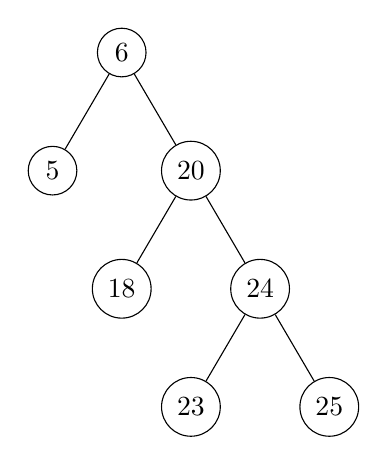
\begin{tikzpicture}
[sibling distance=50,
every node/.style = {shape=circle, draw, align=center}]

\node {6}
child { node {5}}
child { node {20}
	child { node {18}}
	child { node {24}
		child { node {23}}
		child { node {25}}
	}
}
;
\end{tikzpicture}


% Advanced "Binary" Tree with special properties for every level
% Circle objects, everything centered, level based distance between siblings

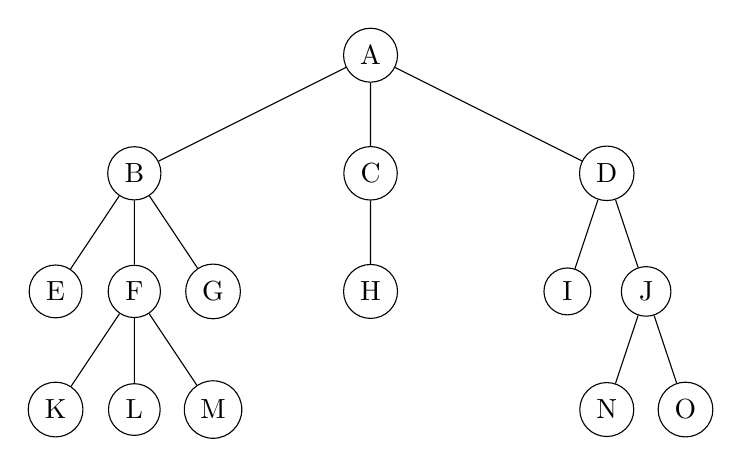
\begin{tikzpicture}
[every node/.style={shape=circle,draw,align=center},
level 1/.style={sibling distance=30mm},
level 2/.style={sibling distance=10mm}]

\node {A}
child { node {B}
	child { node {E} }
	child { node {F}
		child { node {K} }
		child { node {L} }
		child { node {M} }
	}
	child { node {G} }
}
child { node {C}
	child {node {H}}
}
child { node {D}
	child {node {I}}
	child {node {J}
		child {node {N}}
		child {node {O}}
	}
}
;
\end{tikzpicture}

	
}\pdfpageheight=\dimexpr\ht0+\dp0\relax\pdfpagewidth=\wd0\shipout\box0\stop